\ofjob{Warrior}
{
	\ofquote{"I dreamt I was a moron."\\}{Squall}\\\\
	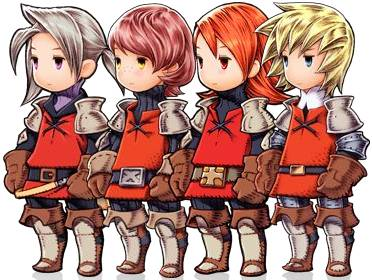
\includegraphics[width=\columnwidth]{./art/jobs/warrior.jpg}\ofrow
	\accf{Warriors} are specialists in melee combat, because of their strong physical offense and defense. 
	They are proficient with powerful swords and armor, allowing them to become even more dangerous and durable. 
%	In his pursuit of ever stronger opponents, the experienced Warrior knows that there is always a bigger fish.
}
{Sword}{Light or Heavy Armor}{
	Level 1: & HP +25 & MP~+18 & AGI~+3 & STR +1 \\
	Level 2: & HP~+10 & MP~+5  & STR~+1 & DEF~+1 \\
	Level 3: & \multicolumn{3}{l}{Archetype Attribute Bonus}  \\
	Level 4: & HP~+10 & MP~+5  & STR~+2 &        \\ 
	Level 5: & HP~+10  & MP~+10 & DEF~+1 \\ 
	Level 6: & HP~+10 & MP~+5  & DEF~+1 & RES~+1 \\ 
	Level 7: & HP~+10 & MP~+10  & STR~+1 &        \\ 
	Level 8: & HP~+10 & MP~+5  & RES~+2 &        \\ 
	Level 9: & HP~+5  & MP~+10 & STR~+1 & DEF~+1 \\ 
	Level 10:& HP~+10 & MP~+5  & DEF~+2 &         
}{
	\ofjobtech{Rush}{3}{0r}{Single}{1u}{Make an Attack against the target. If you hit, you push him back by 1u on top of the damage dealt.}{}{1}\ofabilitygap
	\ofjobtech{Beatdown}{5}{0r}{Single}{1u}{Make an Attack where the target has Advantage on the evasion check. If you hit, you score a Critical Hit.}{}{2}\ofabilitygap
	\ofjobtech{Vitality}{4}{0r}{Single}{Self}{For the next 3 rounds, when an effect restores your HP or MP, the amount is doubled.}{}{4}\ofabilitygap
	\ofjobtech{Army of One}{10}{0r}{3u}{Self}{Make an Attack against every enemy in the target area by making one damage roll that applies to all affected targets that fail to evade. After using the ability, you can move next to any of the affected targets.}{}{6}\ofabilitygap
	\ofjobtech{Bravery}{10}{0r}{2u}{Self}{You and all allies within the target area gain EnSTR and EnMAG for 2 rounds.}{\enstr \enmag}{8}\ofabilitygap
	\ofjobtech{Omnislash}{28}{0r}{Single}{1u}{Make 3 separate Attacks against the target. Each time he rolls 4 or less on an evasion check, you score a Critical Hit.}{}{10}
}{
	\ofarchetypet{Dark Knight}
	{HP~+5 & MP~+15 & DEF~+1 & RES~+2}
	{\ofarchetypetecha{Defensebreak}{6}{0r}{Single}{1u}{Make an Attack on the target. If you hit, he suffers DeDEF and DeRES for 2 rounds on top of the damage dealt. }{\dedef \deres}}
	{\ofarchetypepassive{Souleater}{Whenever you successfully Attack an enemy, you can additionally inflict dark damage equal to half of the total damage dealt, to yourself and all enemies within~3u.}}
	{\ofarchetypereaction{Blood Price}{Whenever an enemy that you can see spends MP, you can force him to spend an equal amount of HP instead if he has enough HP to do so. Afterwards, increase your own HP by half the amount spent.}}
	{\ofarchetypetechb{Berserk}{12}{0r}{Single}{5u}{For the next 3 rounds the target can only take the Attack action, but every successful Attack is a Critical Hit. If you target an enemy with this ability, he makes a DC~8 check and only suffers this effect upon failure.}{}}
}{
	\ofarchetypet{Samurai}
	{HP~+16 & MP~+9 & STR~+2}
	{\ofarchetypetecha{Focus}{5}{0r}{Target}{Self}{For the next 3 rounds, whenever you Attack an enemy, he has Disadvantage on the the evasion check.}{}}
	{\ofarchetypepassive{Cripple}{Whenever the target of your Attacks rolls a 5 or less on the evasion check he additionally suffers one of the following Status Effects of your choice for 1 round upon failure: Immobile, Blind, DeSTR.}}
	{\ofarchetypereaction{Bushido}{You can evade Techs by passing an evasion check the same way that you evade Attacks. Also, whenever you evade an Attack or Tech, you regain an amount of MP equal to your current Level.}}
	{\ofarchetypetechb{Razor Gale}{8}{0r}{5u (line)}{Self}{Everyone in the target area suffers 4d wind damage.}{\wind}}
}